% This must be in the first 5 lines to tell arXiv to use pdfLaTeX, which is strongly recommended.
\pdfoutput=1
% In particular, the hyperref package requires pdfLaTeX in order to break URLs across lines.

\documentclass[11pt]{article}

% Remove the "review" option to generate the final version.
\usepackage[]{acl}

% Standard package includes
\usepackage{times}
\usepackage{latexsym}
\usepackage{booktabs}
\usepackage{url}

%graphics package
\usepackage{graphicx}
\graphicspath{ {./figures/} }

% For proper rendering and hyphenation of words containing Latin characters (including in bib files)
\usepackage[T1]{fontenc}
% For Vietnamese characters
% \usepackage[T5]{fontenc}
% See https://www.latex-project.org/help/documentation/encguide.pdf for other character sets

% This assumes your files are encoded as UTF8
\usepackage[utf8]{inputenc}

% This is not strictly necessary, and may be commented out,
% but it will improve the layout of the manuscript,
% and will typically save some space.
\usepackage{microtype}

% If the title and author information does not fit in the area allocated, uncomment the following
%
%\setlength\titlebox{<dim>}
%
% and set <dim> to something 5cm or larger.

\title{HEVS-TUW at SemEval-2023 Task 8}

% Author information can be set in various styles:
% For several authors from the same institution:
% \author{Author 1 \and ... \and Author n \\
%         Address line \\ ... \\ Address line}
% if the names do not fit well on one line use
%         Author 1 \\ {\bf Author 2} \\ ... \\ {\bf Author n} \\
% For authors from different institutions:
% \author{Author 1 \\ Address line \\  ... \\ Address line
%         \And  ... \And
%         Author n \\ Address line \\ ... \\ Address line}
% To start a seperate ``row'' of authors use \AND, as in
% \author{Author 1 \\ Address line \\  ... \\ Address line
%         \AND
%         Author 2 \\ Address line \\ ... \\ Address line \And
%         Author 3 \\ Address line \\ ... \\ Address line}


\author{Anjani Dhrangadhariya\hspace{1pt}$^{{{\bf 1,2}}\dag}$ \hspace{.7cm} Wojciech Kusa\hspace{1pt}$^{{\bf 3}\dag}$ \\[0.15cm] {\bf Henning Müller\hspace{1pt}$^{{\bf 1,2}}$}  \hspace{.7cm}  {\bf Allan Hanbury\hspace{1pt}$^{{\bf 3}}$}
\\[0.4cm]
{$^1$University of Geneva, Geneva, Switzerland} \\
{$^2$HES-SO Valais-Wallis, Sierre, Switzerland} \\
{\tt \{anjani.dhrangadhariya,henning.mueller\}@hevs.ch} \\
{$^3$TU Wien, Vienna, Austria} \\
{\tt \{wojciech.kusa,allan.hanbury\}@tuwien.ac.at} \\
}


\begin{document}
\maketitle
{\let\thefootnote\relax\footnotetext{$\dag$ Equal contribution.}}

\begin{abstract}
This paper describes the HEVS-TUW team submission to the SemEval-2023 Task 8: Causal Claims.
We participated in two subtasks: (1) causal claims detection and (2)  PIO identification.
For subtask 1, we experimented with an ensemble of weakly supervised question detection and fine-tuned Transformer-based models.
For subtask 2 of PIO frame extraction, we used a combination of deep representation learning and a rule-based approach. 
Our best model for subtask 1 ranks fourth with an F1-score of 65.77\%.
It shows moderate benefit from ensembling models pretrained on independent categories.
The results for subtask 2 warrant further investigation for improvement.
\end{abstract}

\section{Introduction}


\textcolor{red}{1.	Providing a descriptive paper title under the paper template requirement is better. }

\textcolor{red}{2.	I suggest using the combined BiLSTM and CRF architecture to improve the performance for subtask 2.}

% 
Identification and verification of causal claims from unstructured text data is an important task for various decision-making processes, particularly in the field of healthcare. The SemEval-2023 Task 8~\cite{CausalClaims} aims to advance the state-of-the-art in this area by focusing on two subtasks: identification of causal claims and extraction of Population, Intervention, and Outcome (PIO) entities.

% 
The first subtask involves identifying the span of text that contains one of the four entities: a \emph{causal claim}, a \emph{personal experience}, a \emph{personal experience based on a claim} or a \emph{question}. 
This can be done at sentence level, but it is possible that only a part of a sentence is annotated with one of these categories. 
The second subtask involves extracting the PIO frame related to the identified causal claim in a text snippet.
The model utilizes both word-level, including contextual information and character-level features capturing different aspects of the data.


\textcolor{red}{- In the intro, give a short description of your system, without out the conclusions the results/conclusions you present there are uninformative}

Our approach to subtask one fared well at rank~4, with F1-score a 32.77\% better than the last ranked approach and 12.7\% behind the approach ranked~1.
For subtask 2, the approach ranks second last on the leaderboard, and the system mainly struggles with identifying the population frame.
These subtasks have potential applications in content moderation, insurance claim identification, and hypothesis generation from clinical notes.
We believe that the shared task will motivate further research in this direction and lead to the development of more effective and accurate methods for causal claim identification and PIO frame extraction.
%
%
%
\section{Background}
\label{background}
%
%The task of identifying causal claims and extracting the associated PIO frame from unstructured text data has received increasing attention in recent years.
Causal claims identification in the open domain is widely researched, but the healthcare domain has only garnered attention recently~\cite{mueller2018extracting,wang-etal-2019-identifying,parveen-etal-2021-automatic,islam-etal-2021-identifying}.
In the healthcare domain large amounts of medical notes, social media posts, research articles, and patient forums are generated on a daily basis.
Manual extraction of causal claims and PIO frames from such data is a time-consuming and error-prone process.


%Anjani: Background for the PIO extraction task
For a decade, PIO extraction was limited to sentence-level information extraction due to the unavailability of frame-annotated datasets~\cite{boudin2010combining,jin2018pico}.
After the release of the EBM-PICO corpus, the extraction efforts moved to span and frame extraction~\cite{nye2018corpus}.
Nonetheless, previous studies on PIO frame extraction primarily concentrated on extracting them from well-written, peer-reviewed literature~\cite{brockmeier2019improving,zhang2020unlocking,dhrangadhariya2021end}.
The SemEval-2023 task 8 overtakes the challenge of extracting these frames from noisy social media data.
The task organizers provide 597, English-language PIO labelled Reddit posts.
We approach PIO frame extraction as binary sequence labelling and use a combination of deep learning and rule-based approach that captures multiple feature representations from the data, as the dataset is relatively small and noisy.


The SemEval-2023 Task 8 provides an opportunity for researchers to develop novel methods for causal claim identification and PIO frame extraction from noisy social media data and to benchmark their performance against state-of-the-art methods.
We hope that the shared task will lead to the development of more effective and accurate methods for identifying and extracting causal claims and PIO frames from unstructured text data.
%
%
%
\section{System overview}
\label{system_over}
%
We participated in both subtasks of SemEval-2023 Task 8. 
In this section we describe our approach.
%
%
%
\subsection{Subtask 1} \label{sec:system1}
\label{subsec:syst_task1}
%
For subtask 1 we implement two components: weakly supervised question detection and a Transformers-based supervised classifier.
Even though it would be possible to classify the sentences on a sentence-level, we decided to conduct more fine-grained token-level classification.

\subsubsection*{Question detector}


We design a weakly supervised question detector approach (QD).
We use a spaCy sentencizer to split the text into sentences.
Next we search for the occurrences of the question mark token `?' and we assign it an end token of a question span.
To find the beginning span, we either look for a punctuation token from `.’, `!’, `?’ or a token in `how’, ‘what’, ‘where’, `why’.


% 2. weakly questions: st1\_test\_predictions.csv (different folder)

\subsubsection*{Supervised classification}


We fine-tune five models using a training subset of the released dataset:

\begin{enumerate}
\item RoBERTa$_A$ -- RoBERTa model~\cite{Liu2019RoBERTaAR} trained on all entities. % //newstorage5/wkusa/models/pico/ph1-all/roberta/final-model.pt trained for 25 epochs: st1\_test\_flair\_roberta.csv
\item distilBERT$_A$ -- distilBERT model~\cite{Sanh2019DistilBERTAD} trained on all entities.  %all: all\_flair\_submission.csv
\item  distilBERT$_q$ --  distilBERT trained on extracting only questions. %$_q$distil question  question\_flair\_submission.csv
\item distilBERT$_{pe}$ -- distilBERT model trained on personal experience entities %: st1\_test\_flair\_per\_exp.csv
\item distilBERT$_c$ -- distilBERT model trained on claim entities %: st1\_test\_flair\_per\_exp.csv
\end{enumerate}

The three last models are trained as a binary classification. 
For distilBERT$_{pe}$ and distilBERT$_c$, we also assume that all `claims based on personal experience’ tokens are positive for both categories.


%
%
%
\subsection{Subtask 2}
\label{system:task2}
%
PIO extraction was a three-part system: a text preprocessing module, a deep learning entity extraction pipeline and a rule-based approach to combine separate PIO predictions.
%
%
%
\subsubsection{Preprocessing module}
%
The PIO dataset was processed to parse annotation from the Reddit posts.
The empty or partially deleted samples were removed leaving 522 samples.
Next, the text tokens were enriched with the part-of-the-speech (POS) tags and token lemmas using scispaCy\footnote{https://spacy.io/universe/project/scispacy}.
%
%
%
\subsubsection{Deep learning module}
%
The deep learning system was built on combining a feature representation (word-level and character-level) component followed by a linear sequence labelling layer.
We developed our feature representation approach based on the work of Aguilar \textit{et al.}, but with the difference that we did not train our system as a multi-task learning system.
Social media text is highly noisy with writing variations, non-standard abbreviation, spelling errors and grammatically flawed.
Character level representations are useful for capturing the finer details of language, such as spelling variations, unusual short forms, and other non-standard forms of language that are often used in social media. 
Word level representations are important for capturing the overall meaning and context of the language used in social media. 
%Our feature representation approach was inspired from Aguilar \textit{et al.}'s multi-task learning approach~\cite{aguilar2019multi}.
%
%
%
\paragraph{Word-level features: }
%
The word-level features included transformer and POS features.
Transformer models, specifically \textbf{RoBERTa} and \textbf{BioMed-RoBERTa}, were used to extract $\mathbf{T}^{d \times l}$ dimensional contextual features from input samples, where d is the transformer model's hidden layer dimension~\cite{liu2019roberta,gururangan2020don}.
POS information helps NLP models better understand the syntactic structure of a sentence.
The \textbf{POS} embeddings were $\mathbf{P}^{d_p \times 512}$ dimensional one-hot sparse vectors corresponding to the 18-dimensional POS features and the maximum tokens ($l = 512$) allowed per transformer input. 
POS features were either \textbf{one-hot} encoded or transformed using a \textbf{BiLSTM} (bidirectional Long short-term memory) to encode long-term dependencies and learn a task-specific grammatical structure from the input samples~\cite{hochreiter1997long}.
Transformer and POS features were concatenated to obtain a word-level representation (see Figure~\ref{fig:task2_word}).
%Anjani: Include a figure with character and word representations
\begin{figure}[!htbp]
    \centering
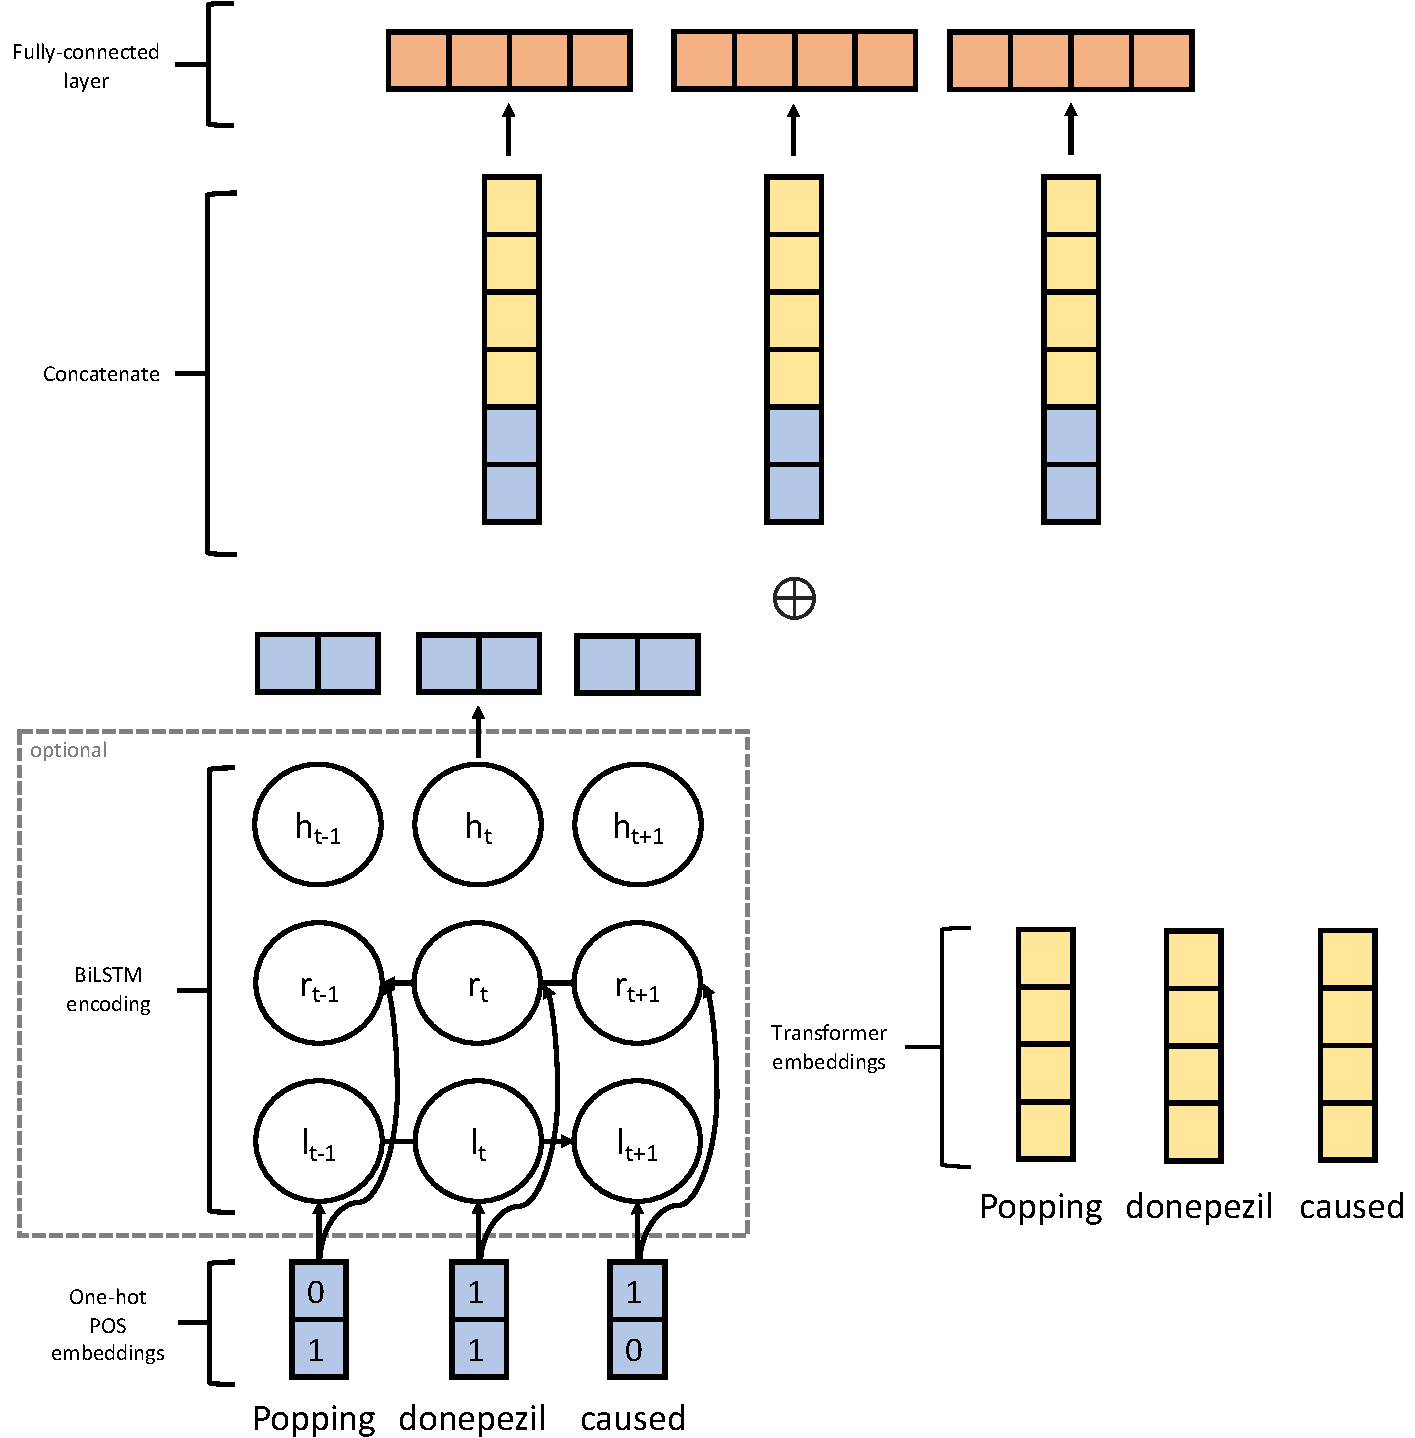
\includegraphics[width=\columnwidth]{figures/word_arch.pdf}
    \caption{Word representation using concatenation of the POS embeddings (in blue, with or without BiLSTM transformation) and transformer embeddings (yellow).}
    \label{fig:task2_word}
\end{figure}
%
%
%
\paragraph{Character-level features: } 
%
To obtain the \textbf{character features}, input characters are embedded into a $\mathbf{C}^{d_{c} \times wl}$ dimensional one-hot encoded vector, where $d_{c}$ is the dimension of the features per character, and $wl$ is the maximum length of characters per word.
\textbf{Orthographic features} are the character-based features $\mathbf{O}^{d_{o} \times wl}$ that encapsulate word shape, including letter capitalization, punctuation, and digits, e.g., "SemEval 2023!" encoded as "CccCccc nnnnp". 
A maximum of 20 characters per token ($wl$) were allowed applying post-padding on shorter tokens and truncating the longer ones.
Character features are matrices encapsulating character-level information, including individual alphabet and punctuation and are hence sparser than the orthographic features.
Our system either used the orthographic or the character features, which were transformed using a 1-dimensional convolutional neural network (\textbf{1D-CNN}) followed by either a max pooling (\textbf{MP}) or global average pooling (\textbf{GAP}) operation~\cite{zhou2016learning}.
Next, the results were fed through a fully-connected (\textbf{fc}) layer via \textbf{ReLU} (Rectified Linear Unit) to obtain a character-level representation (see Figure~\ref{fig:task2_char}).
The final word- and character-level representations were concatenated and fed to a \textbf{linear layer} to predict the entity sequence.
%
%
%
\begin{figure}[!htbp]
    \centering
    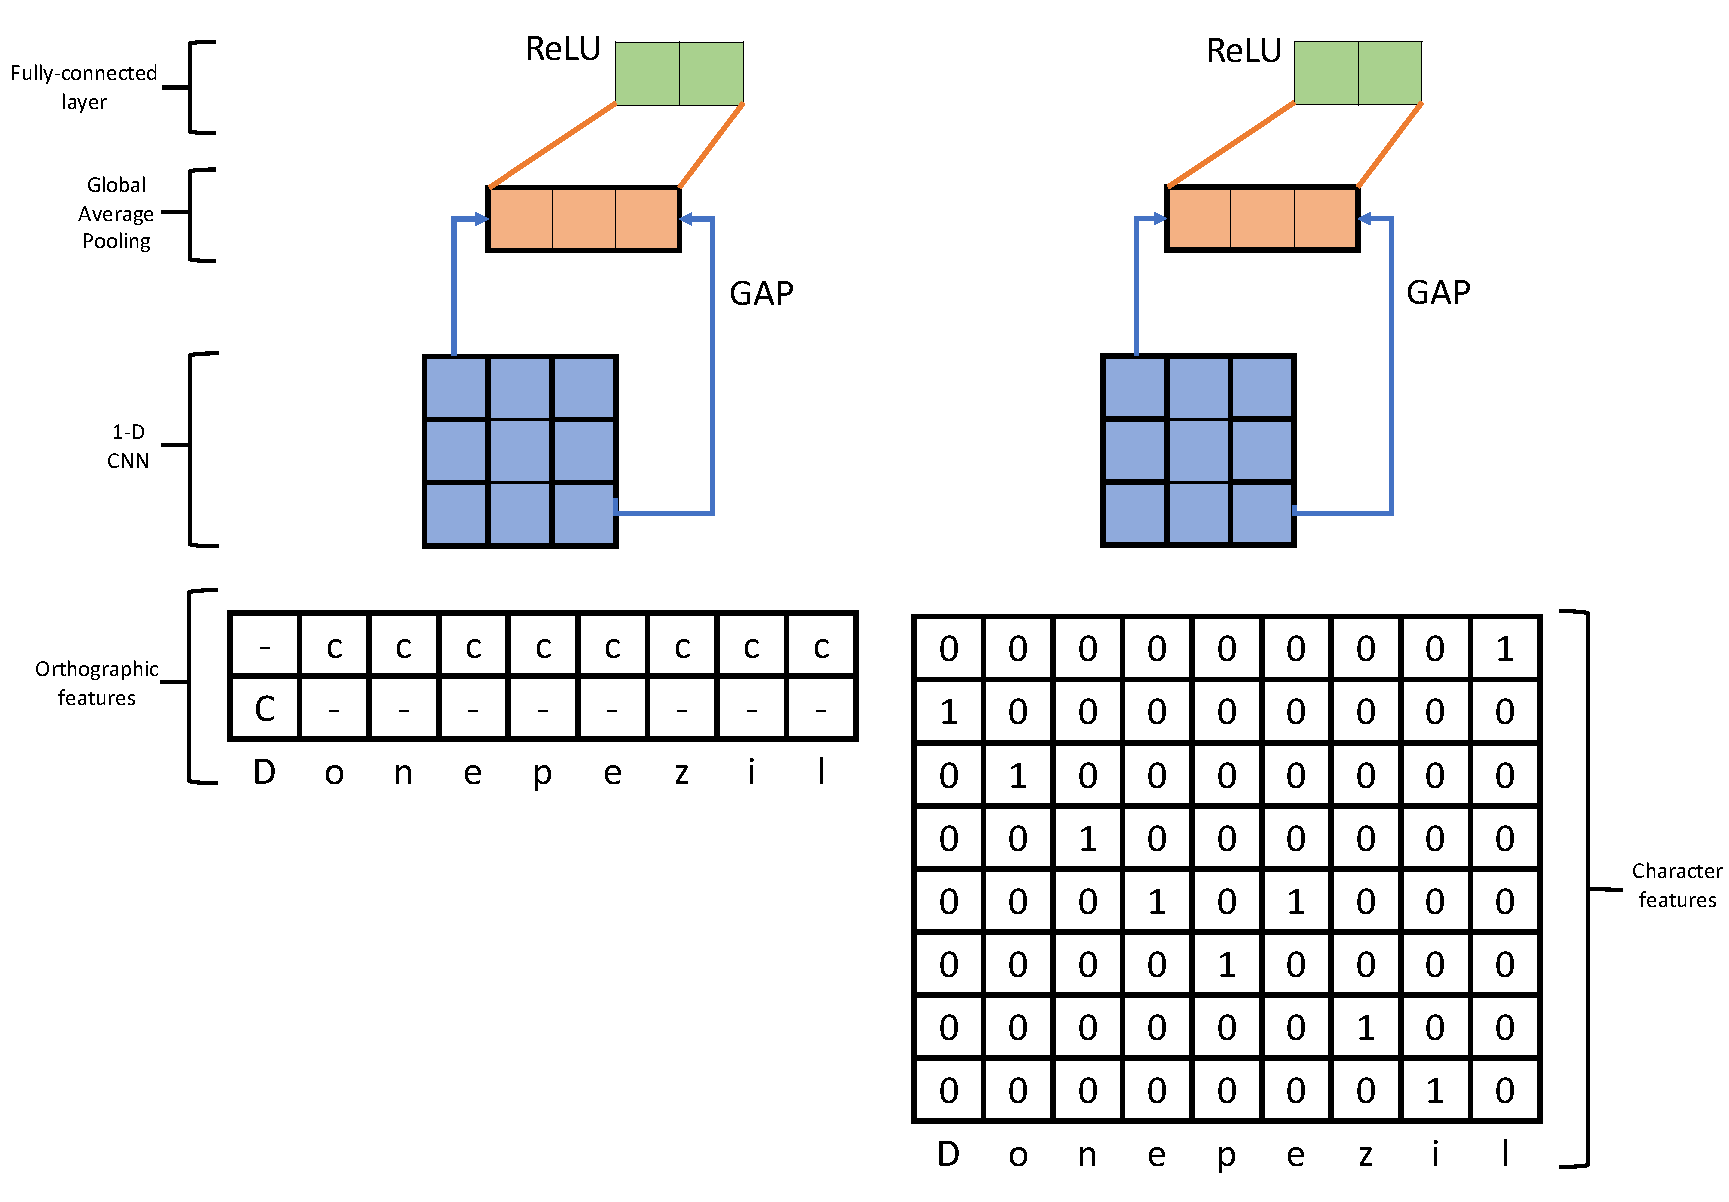
\includegraphics[width=\columnwidth]{figures/word_arch2.pdf}
    \caption{Character representation was was either obtained using the orthographic encoding (left) or character encoding (right) as explained in the system over in section~\ref{system:task2}}
    \label{fig:task2_char}
\end{figure}
%
%
%
\subsubsection{Rule-based module}
%
The processed word and character representations were concatenated and the results were fed to a linear layer to individually predict the PIO entity.
Finally, when multiple predictions were made for the PIO entities, the most common prediction was used, with a random choice being made in case of a tie.
%
%
%
\section{Experimental setup}
This section describes our experimental setup for subtasks (1) and (2), both of which were evaluated using a macro F1-score measure.
%
%
%
% How data splits (train/dev/test) are used.
% Key details about preprocessing, hyperparameter tuning, etc. that a reader would need to know to replicate your experiments. If space is limited, some of the details can go in an Appendix.
% External tools/libraries used, preferably with version number and URL in a footnote.
% Summarize the evaluation measures used in the task.
% You do not need to devote much—if any—space to discussing the organization of your code or file formats.
%
%
%
\subsection{Subtask 1}

We train all Transformer-based models for 30 epochs. 
Following task organizers, we perform splitting on whitespaces.
We use 80\% of the dataset for training models and 20\% for validation.
We use Flair to implement our models~\cite{Akbik2019FLAIRAE}.

For subtask 1 we submit four runs which are ensembles of models described in Section \ref{sec:system1}:

\begin{itemize}
\item \textbf{Run 1:} QD + distilBERT$_q$ + distilBERT$_A$
\item \textbf{Run 2:} QD + distilBERT$_q$ + distilBERT$_{pe}$ + distilBERT$_A$
\item \textbf{Run 3:} QD + distilBERT$_q$ + distilBERT$_{pe}$ + RoBERTa$_A$
\item \textbf{Run 4:} QD + distilBERT$_q$ + distilBERT$_{pe}$ + distilBERT$_A$ + RoBERTa$_A$ 
\end{itemize}

\begin{table}[]
    \centering
    \begin{tabular}{lp{5cm}}
    \toprule
   Run name & Description \\ \midrule
       \textbf{Run 1}  & QD + distilBERT$_q$ + distilBERT$_A$ \\
       \textbf{Run 2}  & QD + distilBERT$_q$ + distilBERT$_{pe}$ + distilBERT$_A$ \\
        \textbf{Run 3} & QD + distilBERT$_q$ + distilBERT$_{pe}$ + RoBERTa$_A$ \\
        \textbf{Run 4} & QD + distilBERT$_q$ + distilBERT$_{pe}$ + distilBERT$_A$ + RoBERTa$_A$ \\
         \bottomrule
    \end{tabular}
    \caption{Caption}
    \label{tab:my_label}
\end{table}

%Run 4 is like Run 2 just adds roberta.
%Run 3 is like Run 2 but last model is switched.
We do the majority voting for non-null predictions, i.e. whenever at least one model predicts an entity, we give that prediction higher precedence compared to a zero-class prediction from other models.
When at least one model predicts the `claim’ category and at least one predicts `personal experience’ we assign to that token the `claim based on personal experience’ entity.
We did not submit a run with distilBERT$_c$ model, as this model was not able to predict any entity correctly on a validation set.

%Runs are evaluated using macro F1-score measure. %Anjani: moved this sentence above as macro F1 was used for both the subtasks and was redundant. 
%
%
%
\subsection{Subtask 2}
\label{exps:task2}
%
For the subtask 2, the experiments were conducted using PyTorch 1.10, scispaCy 0.4.0, and transformers 4.8.2.

We submitted five runs with three training experiments each for PIO classes using the system components described in section~\ref{system:task2}.
For each PIO run, the experiments were conducted and averaged over the three most common Python random seeds, 0, 1 and 42.
The dataset was divided into training (80\%) and validation sets (20\%).
The sequence input length was 512 tokens across the experiments corresponding to the transformer input restriction.
The dimensions for the contextual word embeddings were $\mathbf{T}^{768 \times 512}$ and for the one-hot POS embeddings were $\mathbf{P}^{18 \times 512}$.
The dimensions for the orthographic character embeddings were $\mathbf{O}^{6 \times 20 \times 512}$ and for the character embeddings were $\mathbf{C}^{28 \times 20 \times 512}$.
Specific architecture used for each run is described in the Table~\ref{tab:runs_task2}.
%
\begin{enumerate}
    \item \textbf{Run 1 RoBERTa-(BiLSTM+POS)-(MP(CNN)+fc): } RoBERTa embeddings extracted from the input tokens were concatenated to BiLSTM-transformed POS embeddings to obtain a word-level representation. Character-level orthographic embeddings were CNN transformed, followed by a max pooling operation to obtain the character representation post an fc layer via ReLU.
    \item \textbf{Run 2 RoBERTa-(one-hot-POS)-(MP(CNN)+fc): } RoBERTa embeddings extracted from the input tokens were concatenated to one-hot encoded POS embeddings. Character vectors were CNN transformed, followed by a max pooling operation to obtain the character representation post an fc layer via ReLU.
   \item \textbf{Run 3 RoBERTa-(one-hot-POS)-(GAP(CNN)+fc): } RoBERTa embeddings were concatenated to one-hot encoded POS embeddings. Character-level orthographic embeddings were CNN transformed, followed by a GAP operation to obtain the character representation post an fc layer via ReLU.
   \item \textbf{Run 4 RoBERTa-(BiLSTM+POS)-(GAP(CNN)+fc): } RoBERTa embeddings were concatenated to BiLSTM transformed POS embeddings. Character-level orthographic embeddings were CNN transformed, followed by a GAP operation to obtain the character representation post an fc layer via ReLU.
    \item \textbf{Run 5 Misc:} Three different architectures, each corresponding to PIO classes, were used for the fifth run. For the population class prediction, the architecture was the same as in run 4, except RoBERTa embeddings were replaced by BioMed-RoBERTa representation. For the intervention prediction, the architecture was the same as in run 3, except RoBERTa embeddings were replaced by BioMed-RoBERTa representation. For the prediction of the outcome, only RoBERTa embeddings were extracted from the input tokens, followed by a linear layer for class prediction. 
\end{enumerate}

\begin{table*}[]
    \centering
    \begin{tabular}{lp{13cm}}
    \toprule
   Run name & Model architecture description \\ \midrule
       \textbf{Run 1} & RoBERTa embeddings extracted from the input tokens were concatenated to BiLSTM-transformed POS embeddings to obtain a word-level representation. Character-level orthographic embeddings were CNN transformed, followed by a max pooling operation to obtain the character representation post an fc layer via ReLU. \\
       \textbf{Run 2} & RoBERTa embeddings extracted from the input tokens were concatenated to one-hot encoded POS embeddings. Character vectors were CNN transformed, followed by a max pooling operation to obtain the character representation post an fc layer via ReLU. \\
        \textbf{Run 3} & RoBERTa embeddings were concatenated to one-hot encoded POS embeddings. Character-level orthographic embeddings were CNN transformed, followed by a GAP operation to obtain the character representation post an fc layer via ReLU. \\
        \textbf{Run 4} & RoBERTa embeddings were concatenated to BiLSTM transformed POS embeddings. Character-level orthographic embeddings were CNN transformed, followed by a GAP operation to obtain the character representation post an fc layer via ReLU. \\
        \textbf{Run 5}  & Three different architectures, each corresponding to PIO classes, were used for the fifth run. For the population class prediction, the architecture was the same as in run 4, except RoBERTa embeddings were replaced by BioMed-RoBERTa representation. For the intervention prediction, the architecture was the same as in run 3, except RoBERTa embeddings were replaced by BioMed-RoBERTa representation. For the prediction of the outcome, only RoBERTa embeddings were extracted from the input tokens, followed by a linear layer for class prediction. \\
         \bottomrule
    \end{tabular}
    \caption{The table outlining the model architecture utilized in five different runs for the task of PIO extraction.}
    \label{tab:runs_task2}
\end{table*}

%

%
%
%
\section{Results}
\label{results}
%
%
%
\subsection{Subtask 1}
\label{res:task1}
%
Results for our submissions in subtask 1 are presented in Table \ref{tab:task_1}. 
Adding  distilBERT$_{pe}$ to the ensemble positively impacts Recall and this is the best of our Runs in terms of the F1-score.

\begin{table}[ht]
    \centering
    \begin{tabular}{cccc}
        \toprule
        Run & Precision & Recall & F1-score \\
        \midrule
        1 & 68.13 & 61.21 & 64.48 \\
        2 & 66.81 & \textbf{66.12} & \textbf{66.46} \\
        3 & \textbf{70.32} & 63.38 & 64.52 \\
        4 & 68.73 & 62.90 & 65.70 \\
        \bottomrule
    \end{tabular}
    \caption{Results from subtask 1. \textbf{Bold} values indicate highest score overall.}
    \label{tab:task_1}
\end{table}
%
%
%
\subsection{Subtask 2}
\label{res:task2}
%
Subtask 2 F1-scores for the official SemEval-2023 test set are presented in Table \ref{tab:task_2}.
Run 3 had the best scoring architecture for the mean macro F1 for PIO classes and fared best for intervention and outcome classes.
Run 2 had the best score only for the population class.
Our best F1-score for the task was placed fifth on the leaderboard, 17.91\% points lower than the approach ranked one and 2.52\% better than the last ranked approach.
%
\begin{table}[ht]
    \centering
    \begin{tabular}{ccccc}
        \toprule
          & \multicolumn{4}{c}{Macro F1-acore} \\
         \hline
        Run & Pop & Int & Out & Overall \\
        \midrule
        1 & 12.39 & 19.43 & 22.10 & 17.97 \\
        2 & \textbf{21.30} & 20.05 & 20.33 & 20.56  \\
        3 & 17.44 & \textbf{26.39} & \textbf{22.78} & \textbf{22.20} \\
        4 & 11.54 & 25.63 & 22.74 & 19.97 \\
        5 & 08.18 & 16.47 & 12.28 & 12.31 \\
        \bottomrule
    \end{tabular}
    \caption{Subtask 2 F1-score on the official SemEval-2023 test set for the Population, Intervention and Outcome classes over five runs. Note: Pop = population, Int = intervention, Out = outcome. \textbf{Bold} values indicate highest score overall.}
    \label{tab:task_2}
\end{table}
%
%
%
\section{Conclusion}
%

We participated in both subtasks of SemEval-2023 Task 8.
Our submissions are mainly based on fine-tuning Transformers-based models and creating an ensemble of these models.
Results show a positive impact of using independent models for each entity type in subtask 1.
Source code is available under the following URL: \url{https://github.com/WojciechKusa/pico-semeval2023}
%
%
%
\section*{Limitations}
%
For subtask 2, the rule-based module uses majority voting to choose the final prediction.
MV selects the final token label supported by most of the model runs by equally weighting each run and discounting the accuracy of each model.
The system could benefit from considering model accuracies and weighting predictions from each model to support the final prediction.
Additionally, the final prediction aggregation scheme is stringent and selects only the label predicted by multiple voters.
It could increase the impact of out-of-the-span labels constituting the majority class leading to a lower recall and F1 score.
Consider, for example, only one voter labelling one of the PIO entities and the rest labelling out-of-the-span entity.
For such cases, the rule could be adapted for leniency and selecting the entity in the case at least one voters predict it.
%
%
%
% These instructions are for authors submitting papers to *ACL conferences using \LaTeX. They are not self-contained. All authors must follow the general instructions for *ACL proceedings,\footnote{\url{http://acl-org.github.io/ACLPUB/formatting.html}} and this document contains additional instructions for the \LaTeX{} style files.

% The templates include the \LaTeX{} source of this document (\texttt{acl.tex}),
% the \LaTeX{} style file used to format it (\texttt{acl.sty}),
% an ACL bibliography style (\texttt{acl\_natbib.bst}),
% an example bibliography (\texttt{custom.bib}),
% and the bibliography for the ACL Anthology (\texttt{anthology.bib}).

% \section{Engines}

% To produce a PDF file, pdf\LaTeX{} is strongly recommended (over original \LaTeX{} plus dvips+ps2pdf or dvipdf). Xe\LaTeX{} also produces PDF files, and is especially suitable for text in non-Latin scripts.

% \section{Preamble}

% The first line of the file must be
% \begin{quote}
% \begin{verbatim}
% \documentclass[11pt]{article}
% \end{verbatim}
% \end{quote}

% To load the style file in the review version:
% \begin{quote}
% \begin{verbatim}
% \usepackage[review]{acl}
% \end{verbatim}
% \end{quote}
% For the final version, omit the \verb|review| option:
% \begin{quote}
% \begin{verbatim}
% \usepackage{acl}
% \end{verbatim}
% \end{quote}

% To use Times Roman, put the following in the preamble:
% \begin{quote}
% \begin{verbatim}
% \usepackage{times}
% \end{verbatim}
% \end{quote}
% (Alternatives like txfonts or newtx are also acceptable.)

% Please see the \LaTeX{} source of this document for comments on other packages that may be useful.

% Set the title and author using \verb|\title| and \verb|\author|. Within the author list, format multiple authors using \verb|\and| and \verb|\And| and \verb|\AND|; please see the \LaTeX{} source for examples.

% By default, the box containing the title and author names is set to the minimum of 5 cm. If you need more space, include the following in the preamble:
% \begin{quote}
% \begin{verbatim}
% \setlength\titlebox{<dim>}
% \end{verbatim}
% \end{quote}
% where \verb|<dim>| is replaced with a length. Do not set this length smaller than 5 cm.

% \section{Document Body}

% \subsection{Footnotes}

% Footnotes are inserted with the \verb|\footnote| command.\footnote{This is a footnote.}

% \subsection{Tables and figures}

% See Table~\ref{tab:accents} for an example of a table and its caption.
% \textbf{Do not override the default caption sizes.}

% \begin{table}
% \centering
% \begin{tabular}{lc}
% \hline
% \textbf{Command} & \textbf{Output}\\
% \hline
% \verb|{\"a}| & {\"a} \\
% \verb|{\^e}| & {\^e} \\
% \verb|{\`i}| & {\`i} \\ 
% \verb|{\.I}| & {\.I} \\ 
% \verb|{\o}| & {\o} \\
% \verb|{\'u}| & {\'u}  \\ 
% \verb|{\aa}| & {\aa}  \\\hline
% \end{tabular}
% \begin{tabular}{lc}
% \hline
% \textbf{Command} & \textbf{Output}\\
% \hline
% \verb|{\c c}| & {\c c} \\ 
% \verb|{\u g}| & {\u g} \\ 
% \verb|{\l}| & {\l} \\ 
% \verb|{\~n}| & {\~n} \\ 
% \verb|{\H o}| & {\H o} \\ 
% \verb|{\v r}| & {\v r} \\ 
% \verb|{\ss}| & {\ss} \\
% \hline
% \end{tabular}
% \caption{Example commands for accented characters, to be used in, \emph{e.g.}, Bib\TeX{} entries.}
% \label{tab:accents}
% \end{table}

% \subsection{Hyperlinks}

% Users of older versions of \LaTeX{} may encounter the following error during compilation: 
% \begin{quote}
% \tt\verb|\pdfendlink| ended up in different nesting level than \verb|\pdfstartlink|.
% \end{quote}
% This happens when pdf\LaTeX{} is used and a citation splits across a page boundary. The best way to fix this is to upgrade \LaTeX{} to 2018-12-01 or later.

% \subsection{Citations}

% \begin{table*}
% \centering
% \begin{tabular}{lll}
% \hline
% \textbf{Output} & \textbf{natbib command} & \textbf{Old ACL-style command}\\
% \hline
% \citep{Gusfield:97} & \verb|\citep| & \verb|\cite| \\
% \citealp{Gusfield:97} & \verb|\citealp| & no equivalent \\
% \citet{Gusfield:97} & \verb|\citet| & \verb|\newcite| \\
% \citeyearpar{Gusfield:97} & \verb|\citeyearpar| & \verb|\shortcite| \\
% \hline
% \end{tabular}
% \caption{\label{citation-guide}
% Citation commands supported by the style file.
% The style is based on the natbib package and supports all natbib citation commands.
% It also supports commands defined in previous ACL style files for compatibility.
% }
% \end{table*}

% Table~\ref{citation-guide} shows the syntax supported by the style files.
% We encourage you to use the natbib styles.
% You can use the command \verb|\citet| (cite in text) to get ``author (year)'' citations, like this citation to a paper by \citet{Gusfield:97}.
% You can use the command \verb|\citep| (cite in parentheses) to get ``(author, year)'' citations \citep{Gusfield:97}.
% You can use the command \verb|\citealp| (alternative cite without parentheses) to get ``author, year'' citations, which is useful for using citations within parentheses (e.g. \citealp{Gusfield:97}).

% \subsection{References}

% \nocite{Ando2005,borschinger-johnson-2011-particle,andrew2007scalable,rasooli-tetrault-2015,goodman-etal-2016-noise,harper-2014-learning}

% The \LaTeX{} and Bib\TeX{} style files provided roughly follow the American Psychological Association format.
% If your own bib file is named \texttt{custom.bib}, then placing the following before any appendices in your \LaTeX{} file will generate the references section for you:
% \begin{quote}
% \begin{verbatim}
% \bibliographystyle{acl_natbib}
% \bibliography{custom}
% \end{verbatim}
% \end{quote}

% You can obtain the complete ACL Anthology as a Bib\TeX{} file from \url{https://aclweb.org/anthology/anthology.bib.gz}.
% To include both the Anthology and your own .bib file, use the following instead of the above.
% \begin{quote}
% \begin{verbatim}
% \bibliographystyle{acl_natbib}
% \bibliography{anthology,custom}
% \end{verbatim}
% \end{quote}

% Please see Section~\ref{sec:bibtex} for information on preparing Bib\TeX{} files.

% \subsection{Appendices}

% Use \verb|\appendix| before any appendix section to switch the section numbering over to letters. See Appendix~\ref{sec:appendix} for an example.

% \section{Bib\TeX{} Files}
% \label{sec:bibtex}

% Unicode cannot be used in Bib\TeX{} entries, and some ways of typing special characters can disrupt Bib\TeX's alphabetization. The recommended way of typing special characters is shown in Table~\ref{tab:accents}.

% Please ensure that Bib\TeX{} records contain DOIs or URLs when possible, and for all the ACL materials that you reference.
% Use the \verb|doi| field for DOIs and the \verb|url| field for URLs.
% If a Bib\TeX{} entry has a URL or DOI field, the paper title in the references section will appear as a hyperlink to the paper, using the hyperref \LaTeX{} package.

\section*{Acknowledgements}
\label{acknowledgements}
%
This work was supported by the EU Horizon 2020 ITN/ETN on Domain Specific Systems for Information Extraction and Retrieval (H2020-EU.1.3.1., ID: 860721) and HES-SO Valais-Wallis, Sierre, Switzerland.
%
%
%
% Entries for the entire Anthology, followed by custom entries
\bibliography{anthology,custom}
\bibliographystyle{acl_natbib}

% \appendix

% \section{Example Appendix}
% \label{sec:appendix}

% This is an appendix.

\end{document}
